\chapter*{Management Summary}
	\documentPartEntry{Management Summary}
	
	
	\section*{Ausgangslage}
	
	Die vorliegende Arbeit befasst sich mit der Frage,
	ob und wie sich Aufgaben aus Architekturentscheidungen eines Softwareprojektes teilautomatisiert erzeugen lassen.
	
	Jedes Projekt erfordert das Treffen von Entscheidungen.
	So führt die Entscheidung "<Welche Art Session State soll verwendet werden?"> zum Beispiel zu den Aufgaben
	"<Session State evaluieren"> und "<Prototyp umsetzen">.
	Wird bei dieser Entscheidung die Option "<Database Session State"> ausgewählt,
	so resultieren aus diesem Entscheid beispielsweise die Aufgaben "<Datenbank installieren"> und
		"<Session Persistenz implementieren">.
	
	Sowohl auf Seite der Entscheidungsverwaltung wie auf Seiten der Projektplanungstools existieren bereits verschiedene Tools.
	Ziel von EEPPI ist es, diese Lücke zu schliessen und eine Brücke zwischen Entscheidungsmanagement und Projektplanung zu bilden.
	
	\begin{figure}[H]
		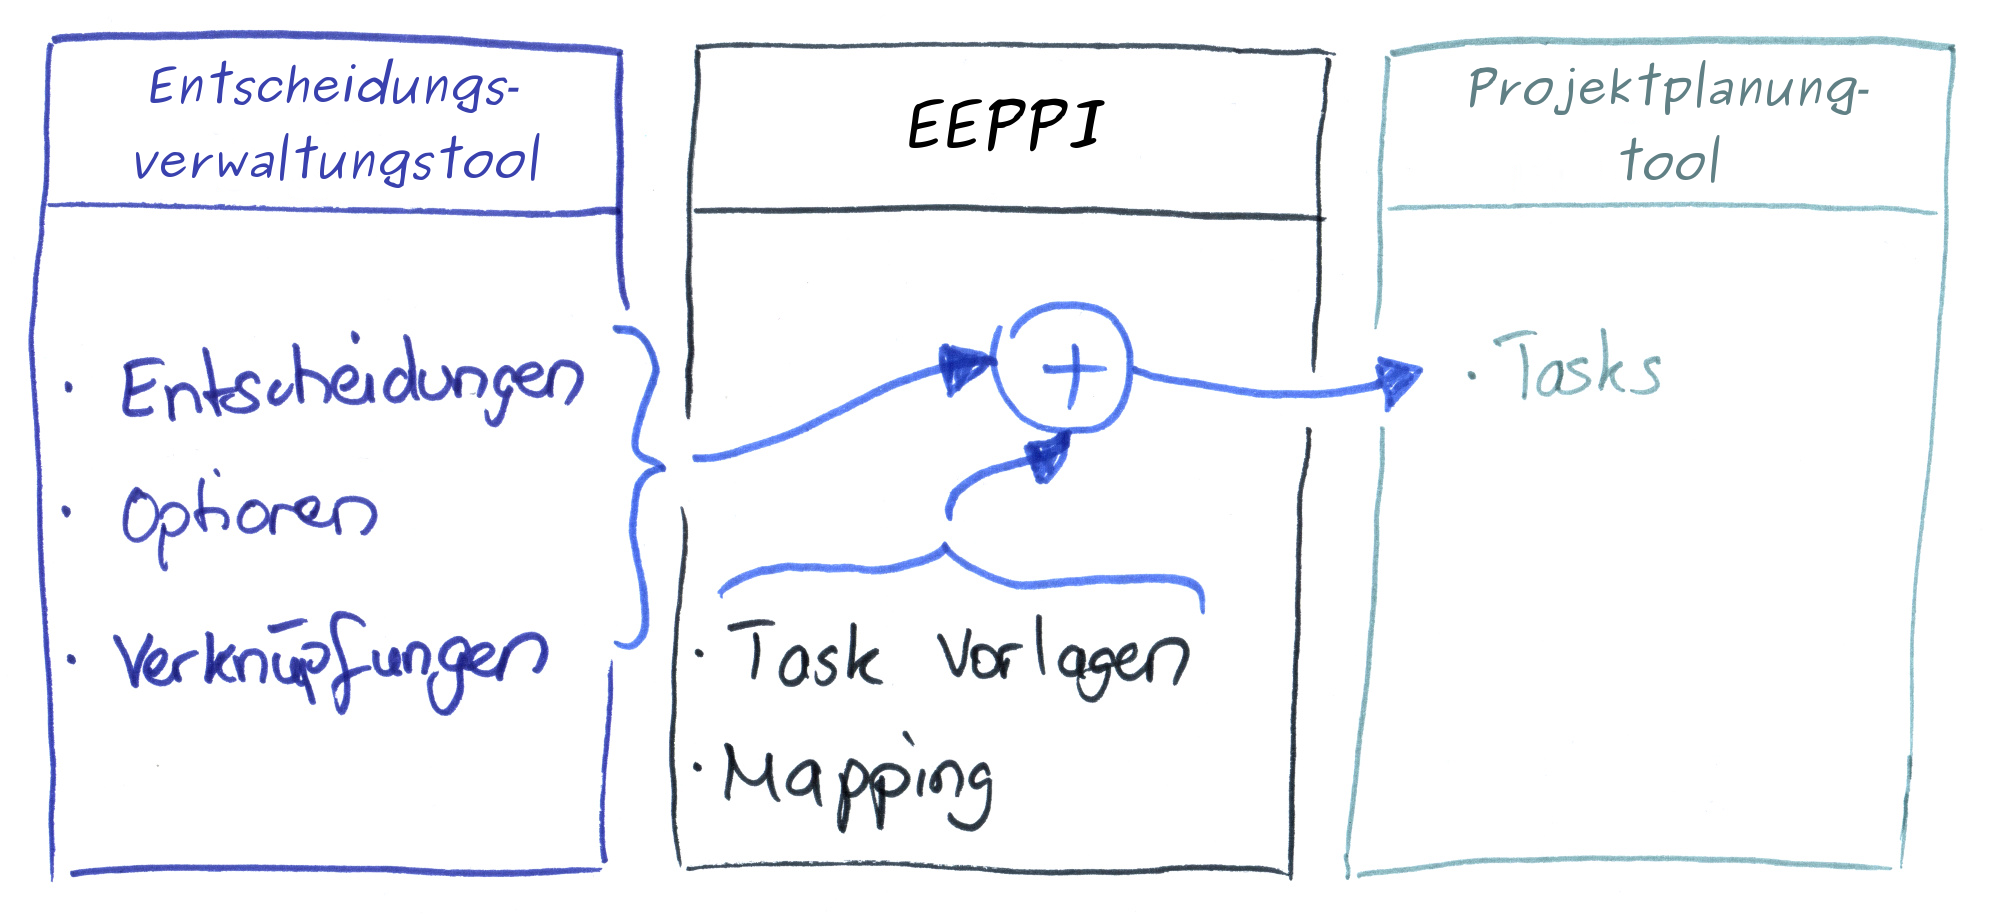
\includegraphics[width=\textwidth]{introduction/img/eeppiVision.png}
		\centering
		\caption{EEPPI bildet eine Brücke zwischen Entscheidungs- und Projektmanagement}
		\label{fig:eeppiBridgeBetweenDecisionsAndTasks}
	\end{figure}
	
	
	\section*{Vorgehen}
	
	Aufbauend auf den Schnittstellen von Wissensverwaltungssystemen und Projektplanungstools wurde eine Applikation entworfen,
	die eine flexible Konfiguration der Schnittstellen ermöglicht.
	Benutzer sollen Aufgabenvorlagen erstellen, diese mit Entscheidungen verknüpfen und in ein Projektplanungstool übertragen können.
	
	Mittels Prototyp wurde die Machbarkeit dessen überprüft
	und anschliessend im Rahmen mehrerer Iterationen eine Webapplikation entwickelt.
	Zusammen mit dem Ansprechpartner der Kundengruppe wurden Usability- und Workflowtests durchgeführt, um Benutzeroberfläche
	und Datenfluss vom Entscheidungsverwaltungssystem bis ins Projektplanungstool zu validieren.
	Abschliessend folgte zur Stabilisierung eine Überarbeitungsphase.
	
	
	\section*{Ergebnis}
		
	Entstanden ist eine Webapplikation, die mögliche Entscheidungen aus einem angebundenen Wissensverwaltungssystem bezieht
	und dem Benutzer durch ein Metamapping ermöglicht, für konkrete Projekte entstehenden Entscheidungen mit eigenen Aufgaben zu Verknüpfen.	
	
	\begin{figure}[H]
		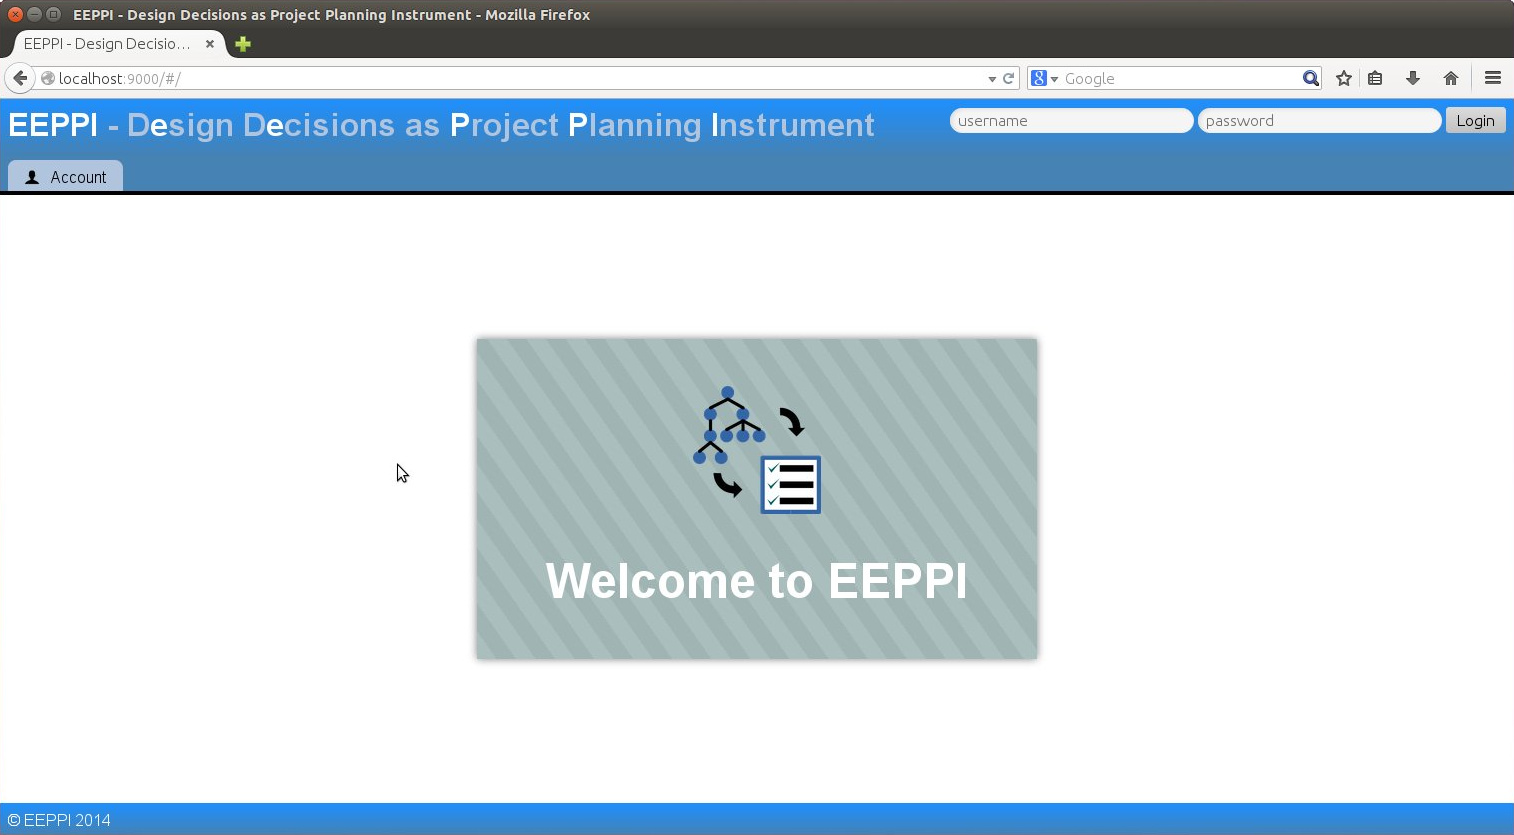
\includegraphics[width=\textwidth]{introduction/img/eeppiDecisionsAndTaskTemplates.jpg}
		\centering
		\caption{Metamapping: Verknüpfung von Entscheidungen und Aufgabenvorlagen}
		\label{fig:metamapping}
	\end{figure}
	
	Über einen  Administrationsbereich konfiguriert der Benutzer die Applikation nach seinen Bedürfnissen.
	Beispielsweise kann der Benutzer selbst den Aufbau der zu generierenden Aufgaben steuern. Dazu wurde ein Templatingmechanismus entwickelt,
	der dem Benutzer das Verwenden von eigenen Verarbeitungsfunktionen, sogenannten Processors, ermöglicht.
	
	EEPPI zeigt, was kommerzielle Produkte in diesem Bereich anbieten könnten.
	Allerdings zeigt EEPPI auch die Design-Herausforderungen einer solchen Software:
	Sowohl die Verknüpfung von Entscheidungen und Aufgaben wie auch die Anbindung an die umliegenden Systeme müssen sehr flexibel gestaltet sein.
	Mit EEPPI ist dies gelungen, doch es gibt noch viele Erweiterungsmöglichkeiten.
	EEPPI legt somit einen wichtigen Meilenstein im Forschungsbereich des interdisziplinären Entscheidungs- und Projektmanagements und
	zeigt auf, wohin die Reise zukünftiger Tools führen könnte.
	
